% !TeX program = xelatex
\documentclass[9pt]{beamer}
\usepackage{xcolor}
\definecolor{orange}{HTML}{FF1053}
\definecolor{lightgray}{HTML}{CCCCCC}
\definecolor{red}{HTML}{AC454A}
\definecolor{brown}{HTML}{EAD296}
\definecolor{darkgrey}{HTML}{313630}
\definecolor{cornflower}{HTML}{247BA0}
\definecolor{sienna}{HTML}{6C464F}
\usefonttheme{professionalfonts} % using non standard fonts for beamer
\usefonttheme{serif} % default family is serif
\usepackage{fontspec}
\usepackage{setspace}
\usepackage{natbib}
\usepackage{animate}
\usepackage{graphicx}
%\usepackage[T1]{fontenc}

\bibliographystyle{abbrv}
%\setmainfont{Liberation Serif}
%\setmainfont{Liberation Serif}
\setmainfont{Comfortaa}
%\usepackage[T1]{fontenc}

\setbeamercolor{frametitle}{bg=orange,fg=white}
\setbeamercolor{author in head/foot}{bg=orange,fg=white}

%\setbeamerfont{page number}{size=\Huge}

%\setbeamertemplate{itemize itemjpegs}[circle]
\useinnertheme{circles}
\setbeamercolor{palette primary}{bg=orange,fg=white}
%\setbeamercolor{palette secondary}{bg=red,fg=white}
\setbeamertemplate{itemize item}{\color{darkgrey}$\circ$}
\setbeamercolor{structure}{fg=darkgrey} % itemize, enumerate, etc

%\setbeamercolor{section in head/foot}{bg=red}
\setbeamercolor{title}{fg=orange} %, bg=brown
\setbeamercolor{author}{fg=darkgrey}
\setbeamercolor{institute}{fg=darkgrey}
\setbeamercolor{date}{fg=darkgrey}
%\setbeamercolor{normal text}{fg=darkgrey}
\makeatletter
\setbeamertemplate{headline}{%
	\usebeamercolor[bg]{frametitle}\rule{\textwidth}{1cm}
}
\setbeamerfont{title}{size=\LARGE}
\setbeamerfont{institute}{size=\normalsize}
\renewcommand*{\bibfont}{\scriptsize}


\setbeamertemplate{frametitle}{%
	\vskip-1cm%
	\begin{minipage}[c][\headheight][c]{\textwidth}%
		\usebeamerfont{frametitle}
		\strut\insertframetitle\par
		{%
			\ifx\insertframesubtitle\@empty%
			\else%
			{\usebeamerfont{framesubtitle}\usebeamercolor[fg]{framesubtitle}\strut\insertframesubtitle\par}%
			\fi
		}%      
		\vspace*{0.05cm}
	\end{minipage}%
	\vskip-0.1em
}
%\setbeamertemplate{footline}{%
%	\leavevmode%
%	\hbox{\begin{beamercolorbox}[wd=\paperwidth,ht=4.5ex,dp=3.125ex]{author in head/foot}%
%			\usebeamerfont{author in head/foot} bar
%	\end{beamercolorbox}}%
%	\vskip0pt%
%}
\makeatother


\title{Simulation-based Inference \\
	\small Inverting Simulators}
\author{Talk by Stefan Wezel}
\institute{mlcolab @ Tübingen University Cluster of Excellence}
\date{\today}


%\setbeamertemplate{sidebar right}{}
%\setbeamertemplate{footline}{%
%	\hfill\usebeamertemplate***{navigation symbols}
%	\hspace{1cm}\insertframenumber{}}
\setbeamerfont{page number in head/foot}{size=\small}
    \setbeamertemplate{footline}{%
	\raisebox{5pt}{\makebox[\paperwidth]{\hfill\makebox[10pt]{\scriptsize\insertframenumber}}}}
\setbeamertemplate{navigation symbols}{}
%\onehalfspacing
\setstretch{1.3}
\begin{document}
	

\setbeamercolor{background canvas}{bg=white}
\setbeamercolor{normal text}{fg=darkgrey}
\usebeamercolor[fg]{normal text}
\begin{frame}[plain]
	\titlepage
\end{frame} 



\setbeamercolor{background canvas}{bg=white}
\setbeamercolor{normal text}{fg=darkgrey}
\usebeamercolor[fg]{normal text}
\setbeamertemplate{itemize item}{\color{darkgrey}$\circ$}
\begin{frame}
\frametitle{Overview}
\framesubtitle{}
\begin{itemize}
	\item What?
	\item Why?
	\item ABC
	\item SBI
	\item Outlook
\end{itemize}
\end{frame} 




\begin{frame}
\frametitle{What}
\framesubtitle{is Simulation-based Inference?}
\begin{itemize}
	\item If we know generating factors, we can build a simulator
	\item But we want to constrain simulator output on observations from real world
	\item Thus we need realistic values for simulator parameters
	\item -> inverse problem
	\item SBI solvers this inverse problem using Bayesian inference
\end{itemize}
\end{frame} 




\begin{frame}
\frametitle{Why}
\framesubtitle{do we need Simulation-based Inference?}
\begin{itemize}
	\item 
\end{itemize}
\end{frame} 



\begin{frame}
\frametitle{How}
\framesubtitle{Approximate Bayesian Computation}
\begin{itemize}
	\item Finding parameters/posterior over parameters with
	\begin{itemize}
		\item Rejection ABC
		\item Markov Chain Monte Carlo ABC
		\item Sequential Monte Carlo ABC
		\item ...
	\end{itemize}
	\item Problems
	\begin{itemize}
		\item 
	\end{itemize}
\end{itemize}
\end{frame} 






\begin{frame}
\frametitle{How}
\framesubtitle{does Simulation-based Inference work?}
\begin{figure}
	%	\flushright
	%	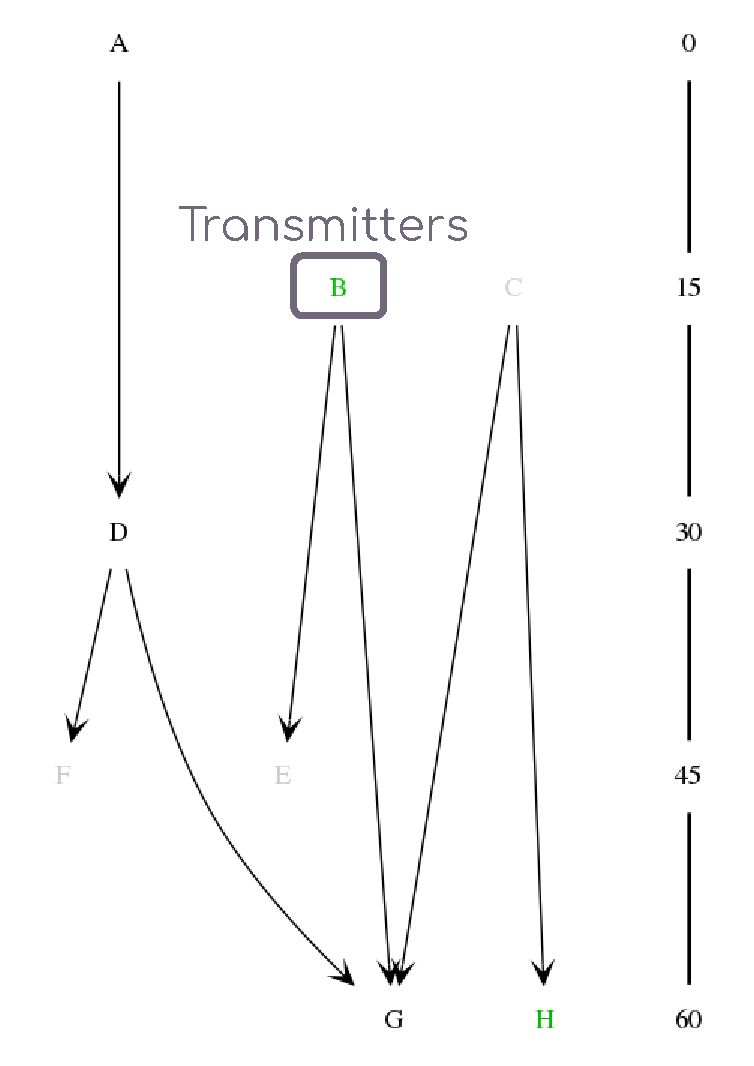
\includegraphics[width=.5\linewidth]{figures/isnalyser_parts_1.pdf}
\end{figure}
\end{frame} 



\end{document}


